\documentclass{standalone}
\usepackage{tikz}
\usepackage{../mss}
\usepackage{sansmath}

\usetikzlibrary{shapes.geometric,positioning,calc,petri,graphs,fit,backgrounds}
\tikzset{
        node distance=1.35cm and 1.35cm,
        >=latex,
        font=\sf\bfseries\sansmath,
        every edge/.append style={line width=1.1pt}
        textfeld/.style={align=center,minimum height=0.5cm,minimum width=1.5cm},
        pfeil/.style={->,line width=1.1pt},
        box/.style={rectangle,draw,line width=1.1pt,minimum height=1.5cm,minimum width=2.8cm,align=center},
        place/.style={circle,line width=1.1pt,draw=black,minimum size=6mm},
        transition/.style={rectangle,line width=1.1pt,draw=black,minimum size=6mm},
        initial/.style={draw=none},
        module/.style={rectangle,fill=gray!5,line width=1.1pt,inner sep=10pt},
        module label/.style={text=gray!50},
        synchronization/.style={draw,dashed,rounded corners,inner sep=6pt},
        segment/.style={rectangle,draw,dashed,rounded corners=3mm,minimum height=1.5cm,minimum width=2.8cm}
        }
\tikzgraphsset{
    every graph/.style = {use existing nodes}
}
\begin{document}
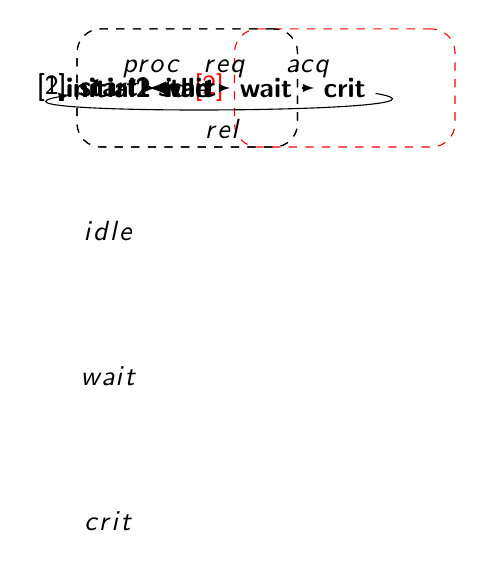
\begin{tikzpicture}
    \node[] (start) {$start$};
    \node[below=of start] (idle) {$idle$};
    \node[below=of idle] (wait) {$wait$};
    \node[below=of wait] (crit) {$crit$};

    \node[initial, above left=3mm and 1.5mm of start] (initial1) {};
    \node[initial, above left=3mm and 1.5mm of wait] (initial2) {};

    \graph{
    start ->[edge label={$ proc $}] idle ->[edge label={$ req $}] wait ->[edge label={$ acq $}] crit ->[overlay,edge label={$ rel $}, bend left=170] start
    };

    \graph{
    initial1 ->[line width=1.2pt] start
    };

    \graph{
    initial2 ->[line width=1.2pt] wait
    };

    \begin{scope}[on background layer]
        \node[segment, fit=(wait), label={left:$ \segment[2] $}] (o21) {};
        \node[segment, draw=red, fit=(crit), label={left:\textcolor{red}{$ \segment[2] $}}] (o22) {};
        \node[segment, fit=(start) (idle) (wait), label={left:$ \segment[1] $}] (o23) {};
    \end{scope}

\end{tikzpicture}
\end{document}